\PassOptionsToPackage{dvipsnames}{xcolor}
\documentclass[border=3mm]{standalone}
\usepackage[dvipsnames]{xcolor}
\usepackage{amsmath}
\usepackage{amssymb}
\usepackage{dsfont}
\usepackage{bm}
\usepackage{tikz}
\usetikzlibrary{arrows}
\usetikzlibrary{calc}



\definecolor{color1}{rgb}{0,0.4470,0.7410}
\definecolor{color2}{rgb}{0.8500,0.3250,0.0980}
\definecolor{color3}{rgb}{0.9290,0.6940,0.1250}
\definecolor{color4}{rgb}{0.4940,0.1840,0.5560}
\definecolor{color5}{rgb}{0.4660,0.6740,0.1880}


\begin{document}



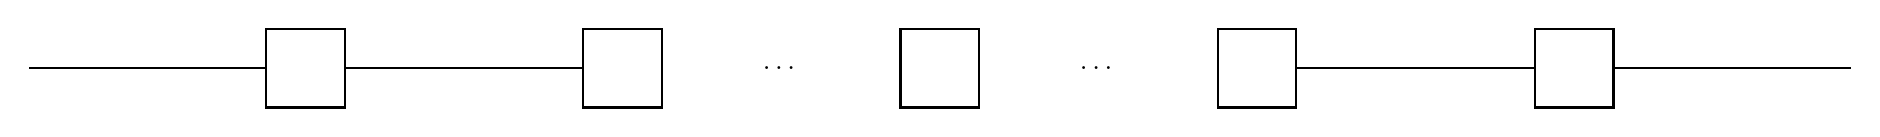
\begin{tikzpicture}[>=stealth,thick]

\node [rectangle, draw, minimum width = 1cm, minimum height = 1cm, anchor=west] (n1) at (0,0) {};
\node [rectangle, draw, minimum width = 1cm, minimum height = 1cm, anchor=west] (n2) at ($(n1.east)+(3,0)$) {};
\node [rectangle, draw, minimum width = 1cm, minimum height = 1cm, anchor=west] (n3) at ($(n2.east)+(3,0)$) {};
\node [rectangle, draw, minimum width = 1cm, minimum height = 1cm, anchor=west] (n4) at ($(n3.east)+(3,0)$) {};
\node [rectangle, draw, minimum width = 1cm, minimum height = 1cm, anchor=west] (n5) at ($(n4.east)+(3,0)$) {};


\draw (n1.west) -- + (-3,0);
\draw (n1.east) --  (n2);

\path (n2.east) -- node {$\dotsc$} (n3) ;
\path (n3.east) -- node {$\dotsc$} (n4) ;

\draw (n4.east) --  (n5);
\draw (n5.east) -- + (3,0);

\end{tikzpicture}

\end{document}
























